\setcounter{section}{4}
\setcounter{subsection}{4}
\setcounter{equation}{14}

\subsubsection{Mikrowellenspektroskopie}
	Die Mikrowellenspektroskopie wird fast nur mit Absorbtion eingesetzt, weil die Übergangswahrscheinlichkeit für eine spontane Emission sehr klein ist (Einsteinkoeffiezient $A_{21} \sim \omega^3$).
	\autoref{fig:vl08_abbildung_1} zeigt den schematischen Aufbau einer Messvorrichtung.
	\begin{figure}[H]
		\centering
		\incfig{vl08_abbildung_1}
		\caption{Schematische Darstellung einer Messvorrichtung zur Mikrowellenspektroskopie.}
		\label{fig:vl08_abbildung_1}
	\end{figure}

	\begin{verbal}
		In Demtröders \textit{Experimentalphysik 3} werden die Spektroskopiemethoden und die dabei verwendeten Bauteile genauer erklärt.
	\end{verbal}

	Reine Rotationsspektren sind nur für polare Moleküle mit \textbf{permanenten elektrischen Dipolmomenten} beobachtbar.
	Ein Molekül hat dann für einen ortsfesten Beobachter eine veränderliches Dipolmoment: 
	Klassisch betrachtet entspricht die Rotationsfrequenz $\omega_\mathrm{rot}$ des Moleküls der abgestrahlten Lichtfrequenz.
	Quantenmechanisch gilt Fermi's goldene Regel
	$$
	\left| \bra{ \psi_{\text{final }}} \vec{d} \vec{E} \ket{ \psi_{\text{initial }}} \right|^2 \sim f    
	$$
	mit den Kugelflächenfunktionen $ \psi_{\text{final}}$ und $ \psi_{\text{initial}}$, dem Dipolmoment $ \vec{d}$, dem elektrischen Feld $\vec{E}$ und
	der Übergangswahrscheinlichkeit $f$. Beispiele für sollche polaren Moleküle sind \ce{HCl} und \ce{HBr}. Gegenbeispiele sind
	\ce{H2}, \ce{O2} und \ce{N2}, welche Raman-aktiv sind und im MSc-Kurs behandelt werden.

\subsubsection{Zweiatomige Moleküle}
\paragraph{\thesubsubsection.1. Starrer Rotator (Hantel-Modell)}~\\

	Das Zweiatomige Molekül wird zunächst als starrer Rotator gemäß \autoref{fig:vl08_starrer_koerper} betrachtet.
	\begin{figure}[H]
		\centering
		\includegraphics[width=0.5\textwidth]{./figures/VL08_Abbildung_2.tikz}
		\caption{Schema eines starren Rotators mit Massen $m_1$, $m_2$ an den Enden. Der Körper rotiert mit Kreisfrequenz $\omega$ um seinen Schwerpunkt (SP).}
		\label{fig:vl08_starrer_koerper}
	\end{figure}
	\autoref{fig:vl08_starrer_koerper} zeigt die Zusammenhänge
	$$
	\begin{aligned}
		m_1 R_1 = m_2 R_2,\quad
		R = R_1 + R_2\quad\text{und}\quad
		\Theta = m_1 R_1^2 + m_2 R_2^2 = m_{r}R^2
	\end{aligned}
	$$ 
	mit der reduzierten Masse
	$$
	m_{r} = \frac{m_1m_2}{m_1 + m_2}.
	$$ 
	Die Rotationsenergie beträgt
	\begin{equation}
		\label{4.15}
		E_{\text{rot}} = \frac{1}{2} \Theta \omega^2 = \frac{L^2}{2 \Theta}.
	\end{equation} 

	Das System hat den klassischen Drehimpuls
	\begin{equation}
		\label{4.16}
		\left| \Vec{L} \right| = \Theta \omega,
	\end{equation}

	bzw. den quantenmechanischen Drehiumpuls
	\begin{equation}
		\label{4.17}
		\left| \Vec{L} \right| = \sqrt{ J(J+1)} \hbar 
	\end{equation}
	Daraus folgt die quantenmechanische Rotationsenergie
	\begin{equation}
		\label{4.18}
		E_{\text{rot}} = \frac{ \hbar ^2}{2 \Theta} J(J+1) \qquad\text{mit } J \in \{0,1,2,3,\ldots\}.
	\end{equation}

	\begin{definition}{}
		\begin{equation}
			F(J)=\frac{E_\mathrm{rot}}{hc} = BJ(J+1)
		\end{equation}
		mit der \textbf{molekülspezifischen Rotationskonstante} $$B=\frac{h}{8\pi^2c\Theta}$$ des starren Rotators ($[B]=\unit{\per\centi\meter}$).
	\end{definition}
	Die Drehimpulsauswahlregel schreibt vor 
	$$\Delta J = \pm1, \qquad M=J,J-1, \ldots, -J+1, -J.$$
	Daraus folgt
	\begin{equation}
		F(J+1)-F(J) = 2B(J+1) = 2B,~4B,~6B, \ldots
	\end{equation}
	\autoref{fig:spektrum_starrer_rotator} zeigt das entsprechende Energieniveauschema und Spektrum.
	\begin{figure}[H]
		\centering
		\includegraphics[width=0.5\textwidth]{./figures/VL08_Abbildung_3.tikz}
		\caption{Schematisches Energieniveauschema und Spektrum eines zweiatomigen Moleküls, welches als starrer Rotator modelliert wird}
		\label{fig:spektrum_starrer_rotator}
	\end{figure}
	Anmerkungen zum Spektrum:
	\begin{itemize}
		\item die Entartung ist $ 2J+1$-fach
		\item die Rotation um die Verbindungsachse kann nicht angeregt werden, da $ \Theta$ sehr klein ist. Um diese Rotation anzuregen, wären Energien im Bereich $F(J)\gg1\unit{\electronvolt}$ notwendig, welche das Molekül davor zerstören.
		\item Beispielwerte der Rotationskonstante $B$ sind in \autoref{tab:vl08_verschiedene_B} eingetragen.			
	\end{itemize}
	\begin{table}[htpb]
		\centering
		\caption{Molekülspezifische Rotationskonstanten $B$ verschiedener Stoffe.}
		\label{tab:vl08_verschiedene_B}
		\begin{tabular}{|l|c|}
			\hline
			Stoff & $2B$ in $\unit{\centi\meter ^{-1}}$ \\
			\hline
			\ce{HCl} & \num{20,79}\\
			\ce{CO} & \num{3,84}\\
			\ce{HBr}& \num{14,9}\\
			\hline
		\end{tabular}
	\end{table}

	Die Intensitäten der Rotationslinien ergeben sich bei konstantem Übergangs\-matrix\-element aus
	\begin{itemize}
		\item dem Entartungsgrad der Terme $F_{J}$: $g_{J}= 2J+1$ 
		\item der Auswahlregel $ \Delta J = \pm 1$  
		\item der thermische Besetzung der Rotationsniveaus. Diese wird von der Boltzmanverteilung beschrieben. Die thermische Energie bei Raumtemperatur entspricht ca. $\frac{1}{40}\unit{\electronvolt} \simeq \SI{200}{\centi \meter ^{-1}}\gg B$. Es sind bei Raumtemperatur also viele Niveaus besetzt. 
	\end{itemize}
	Aus der Boltzmanverteilung folgt
	\begin{important}
		\begin{equation}
			\frac{N_J}{N_0} = \frac{g_j}{g_0}\mathrm e^{-\frac{E_J-E_0}{k_\mathrm BT}} = (2J+1)\mathrm e^{-\frac{BhcJ(J+1)}{k_\mathrm BT}}.
			\label{eq:4.21}
		\end{equation}
	\end{important}
	Der Verlauf von $N_J/N_0$ ist in \autoref{fig:vl08_NJ-N0_Verlauf} dargestellt.
	\begin{figure}[H]
		\centering
		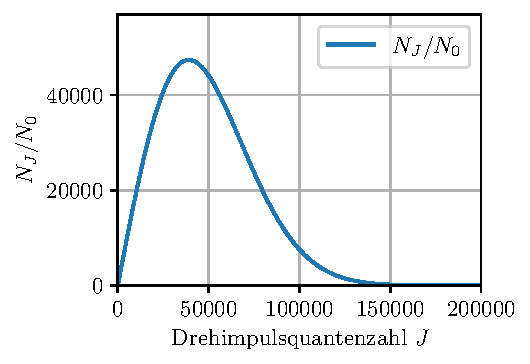
\includegraphics[width=8cm]{figures/vl08/N_verhaeltnis.pdf}
		\caption{Verlauf von $N_J/N_0$ bei Raumtemperatur $T=\SI{293,15}{\kelvin}$. Für kleine Drehimpulse $J$ dominiert der lineare Term $(2J+1)$, für große dominiert die Exponentialfunktion}
		\label{fig:vl08_NJ-N0_Verlauf}
	\end{figure}

	\paragraph{Bemerkungen}
	\begin{itemize}
		\item Auch das Übergangsmatrixelement hängt von $J$ ab wegen den zugehörigen Wellenfunktionen
		$$
		\left| \bra{ \psi_{\text{i}}}  \Vec{d} \Vec{E} \ket{ \psi_{\text{f}}}  \right|^2 
		$$ 
		Das ist im Allgemeinen jedoch nur eine geringfügige Korrektur.

		\item Aus Messungen von $N_J/N_0$m $J$, und $B$ lässt sich nach Gleichung \eqref{eq:4.21} die Temperatur $T$ einer Probe bestimmen.
	\end{itemize}

\paragraph{\thesubsubsection.2. Nichtstarrer Rotator}~\\

	Aus Beobachtungen ergibt sich, dass für große $J$ die Distanz der Linien im Rotationsspektrum enger wird. Die Ursache dafür der wachsende Kernabstand für große $J$ aufgrund der Zentrifugaldehnung

	\textcolor{red}{Abbildung hier}\\
	mit 
	$$
	E_{\text{rot}} = \frac{L^2}{2 \theta}
	$$ 
	Dieser Effekt sit besonders wichtig, wenn zur Rotation auch noch Schwingungen hinzukommen. Klassisch gilt mit der Zentrifugalkraft und der Federkraft
	\begin{equation}
		\label{4.22}
		m_{r}R \omega^2 = K\left( R-R_{e} \right) 
	\end{equation}
	mit dem Gleichgewichtsabstand $e$. Es ist
	\begin{equation}
		\label{4.23}
		\Delta R = R - R_{e} = \frac{m_{r} R \omega^2}{K} = \frac{m_{r}^2 R^{4} \omega^2}{K m_{r} R^3} = \frac{\left( \Theta \omega \right) ^2}{K m_{r} R^3} 
	\end{equation}
	womit
	\begin{equation}
		\label{4.24}
		(R - R_{e} ) = \frac{L^2}{k m_{r} R^3} \simeq \frac{L^2}{km_{r} R_{e}^3}		
	\end{equation}
	folgt, da
	$$
	R^3 = (R + \Delta R)^3 = R_{e} ^3 \left( 1 + \frac{ 3 \Delta R}{R_{e}}+ \ldots \right).
	$$  
	Die Rotationsenergie ist dann $ E_{\text{rot}} = E_{\text{rot}} + E_{\text{spann}}$. Nach klassischer Betrachtung folgt
	$$
	E_{\text{rot}} = \frac{L^2}{2m_{r} R_{e}^2} - \frac{1}{2} K\left( R - R_{e} \right) ^2 = \frac{L^2}{2 m_{r} R_{e}^2} - \frac{L^{4}}{2Km_{r}^2 R_{e}^{6}}
	$$ 
	und nach quantenmechanischer $(L^2 \to  J(J+1) \hbar ^2)$ Betrachtung ergibt sich 
	\begin{equation}
		\label{4.27}
		E_{\text{rot}} = \frac{\hbar ^2}{2 m_{r}R_{e}^2} J\left( J+1 \right) - \frac{\hbar ^{4}}{2 k m_{r}^2 R_{e}^{6}} J^2\left( J+1 \right) ^2 
	\end{equation}

	Für Rotationsterme in \unit{\centi\meter ^{-1}}:
	\begin{equation}
		\label{4.28}
		F(J) = \frac{ E_{\text{rot}}}{\mathrm{hc}} = B J\left( J+1 \right) - DJ^2 \left( J+1 \right) ^2			
	\end{equation}

	Bemerkung:
	$$
	\frac{D}{B} \approx 10^{-4} \text{ bis } 10^{-3} 
	$$
	womit der Dehnungsterm für kleine $J$ vernachlässigbar ist.\\
	Für große $J$ kann man die Federkonstante $k$ der Bindung bestimmen.

	\textcolor{red}{Abbildung hier}

	Auswahlregeln bleiben unverändert $\left( \Delta J = \pm 1 \right) $ da die Symmetrien der Rotationszustände nicht geändert werden
	\begin{equation}
		\label{4.29}
		F(J) - F(J+1) = 2B(J+1) - 4D(J+1)^3
	\end{equation}

	\paragraph{Isotropie-[Effekte}
	$$
	B \sim  \frac{1}{ \Theta}, \quad \Theta = m_{r} R^2
	$$ 
	$\to $ Linienverschiebung für Isotope.
	Bsp. \ce{H2} und schwerer Wasserstoff  $\ce{^1H} \to  \ce{^2H}$. Für das Protium ($\ce{^1H}$ Molekül gilt  $2B = \SI{121,61}{\centi \meter ^{-1}}$, für das Deuterium Molekül hingegen $ 2B = \SI{60,86}{\centi \meter^{-1}}$.
	Bsp.
	$$
	\begin{aligned}
		&\ce{H^{35}Cl} \quad \left( \SI{75}{\percent} \right) \\
		&\ce{H^{37}Cl} \quad \left( \SI{25}{\percent} \right) 
	\end{aligned} \quad
	\frac{ \Delta \nu}{ \nu} = \frac{1}{670} \approx 1\,\text{\textperthousand}
	$$
	d.h. jede Rotationslinie tritt doppelt auf.\\
	Bemerkung:
	\begin{itemize}
		\item Aus $ \Delta \nu$ $ \to $ Isotopenmassen
		\item aus Intensität  $\to $ Isotopenmischung
	\item Bindungsabstände von komplexen Molekülen können bestimmt werden, bspw \ce{OCS} (Kohlenstoffoxysulfid)
	\end{itemize}
